\chapter{Route vers Bangalore}
\section*{15 décembre 2015}
C'est parti pour les 300 derniers km en vélo jusqu'à Bangalore \newline
 \newline
\centerline{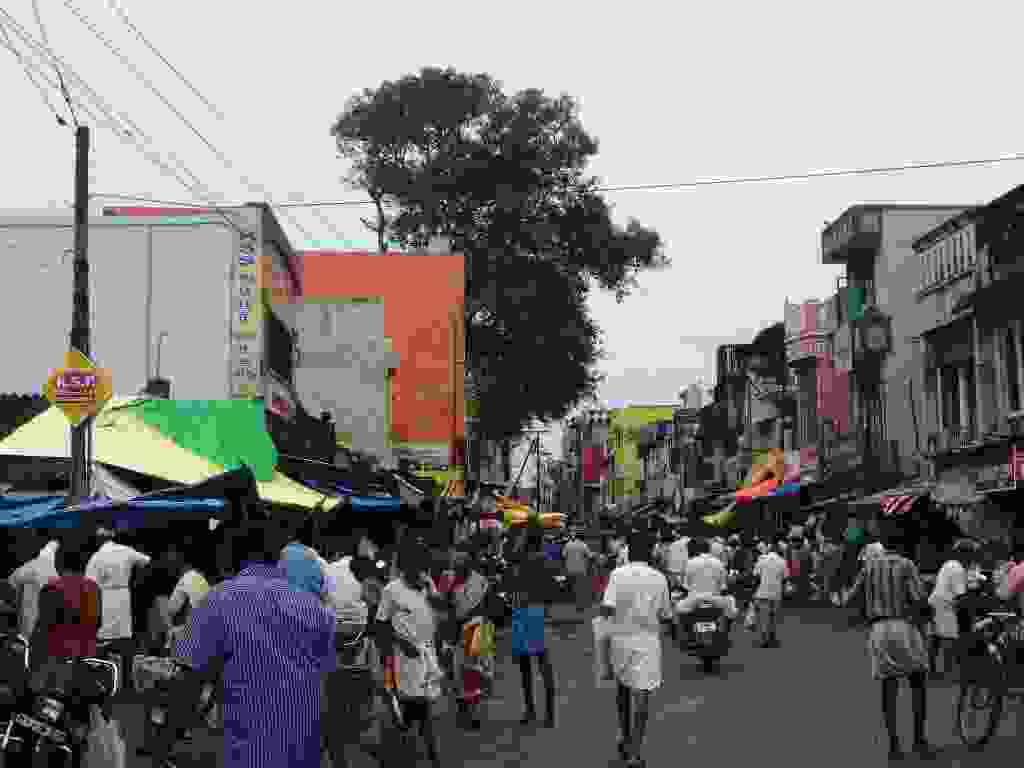
\includegraphics[width=\mywidth]{../wp-content/uploads/2015/12/wpid-oi000646-1024x768.jpg} } 
 \newline
 \newline
\centerline{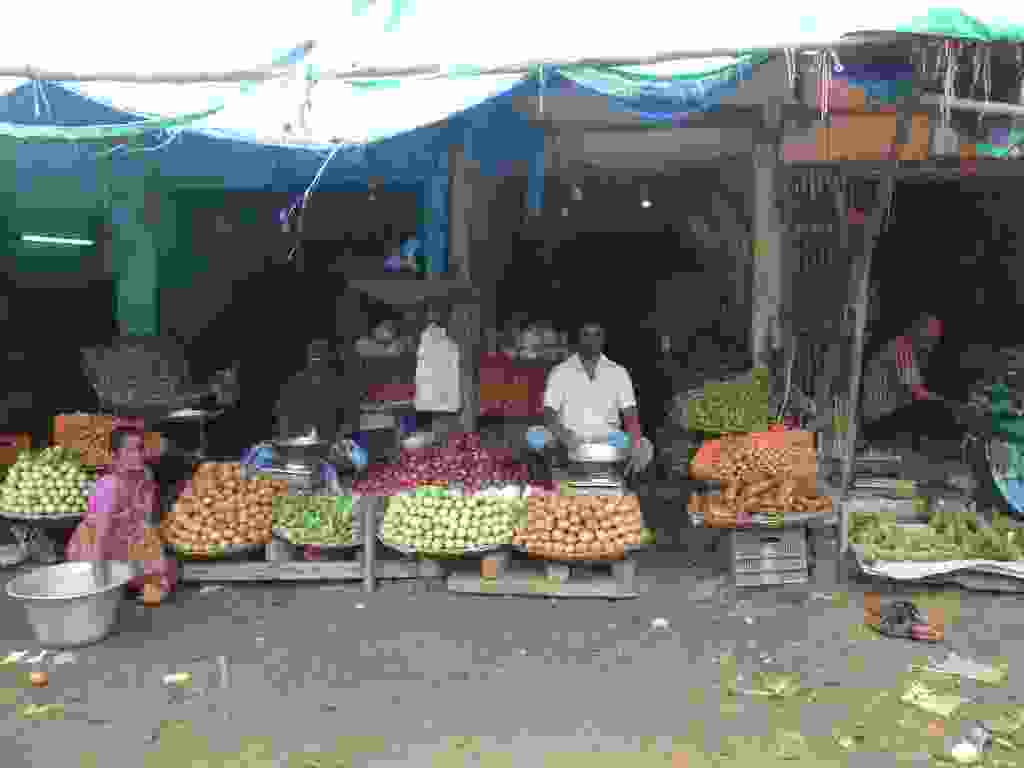
\includegraphics[width=\mywidth]{../wp-content/uploads/2015/12/wpid-oi000648-1024x768.jpg} } 
 \newline
 \newline
\centerline{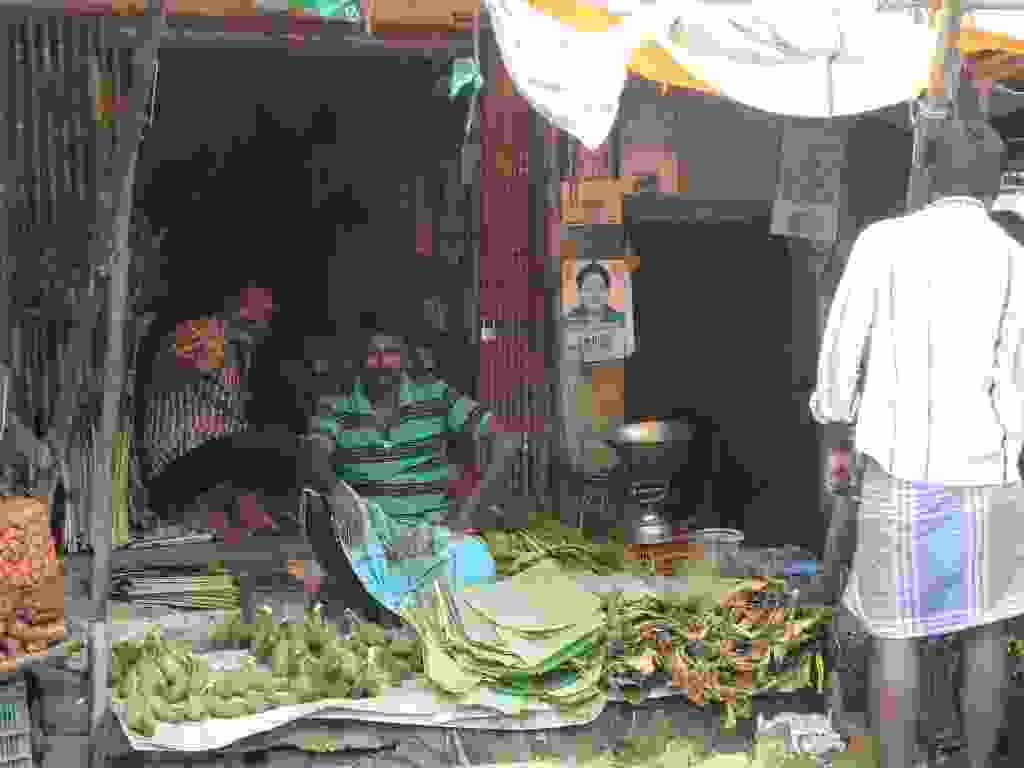
\includegraphics[width=\mywidth]{../wp-content/uploads/2015/12/wpid-oi000649-1024x768.jpg} } 
 \newline
 Passage par Gingee, l'occasion de monter sur l'un des forts de la ville \newline
 \newline
\centerline{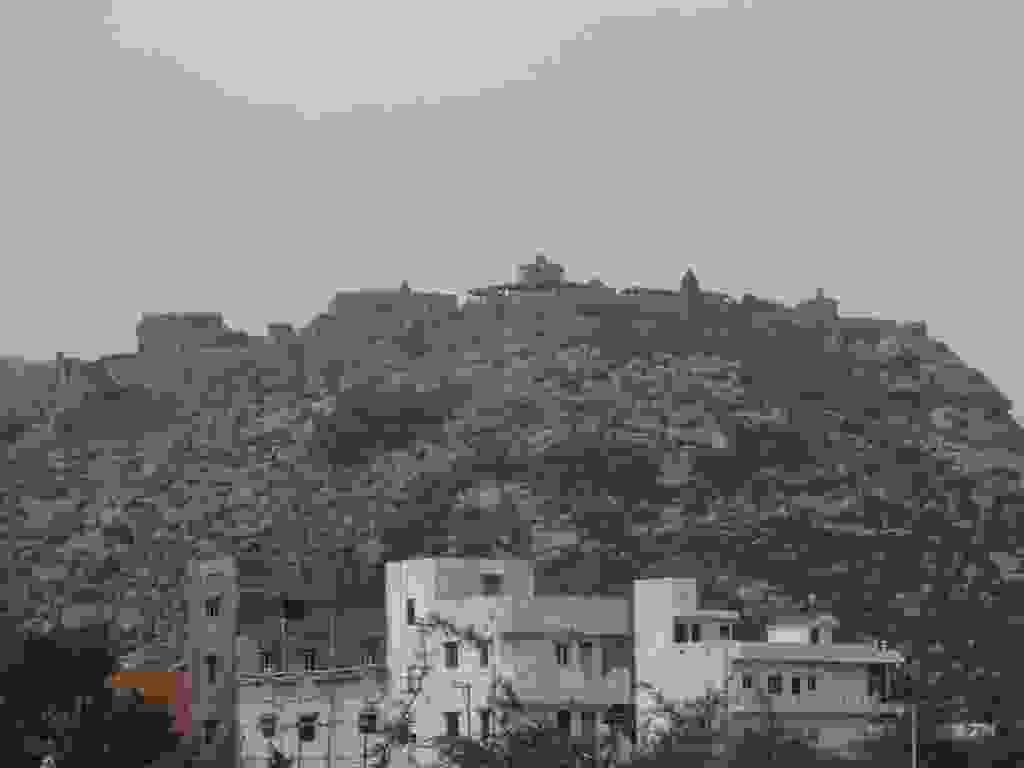
\includegraphics[width=\mywidth]{../wp-content/uploads/2015/12/wpid-oi000656-1024x768.jpg} } 
 \newline
 \newline
\centerline{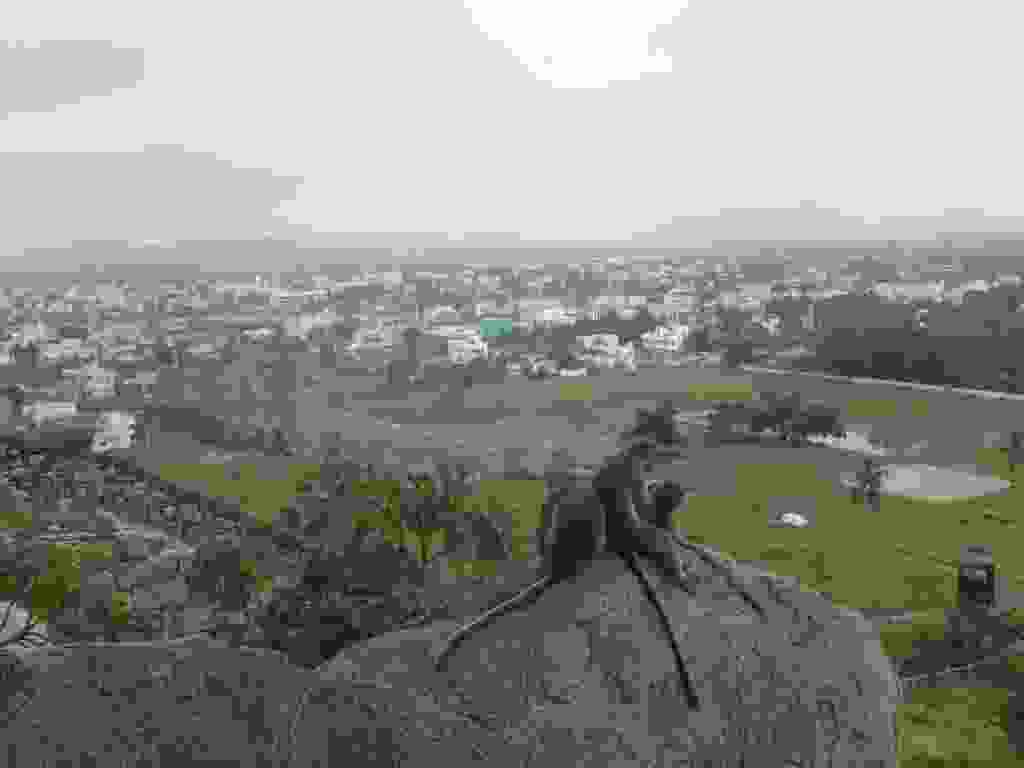
\includegraphics[width=\mywidth]{../wp-content/uploads/2015/12/wpid-oi000665-1024x768.jpg} } 
 \newline
 \newline
\centerline{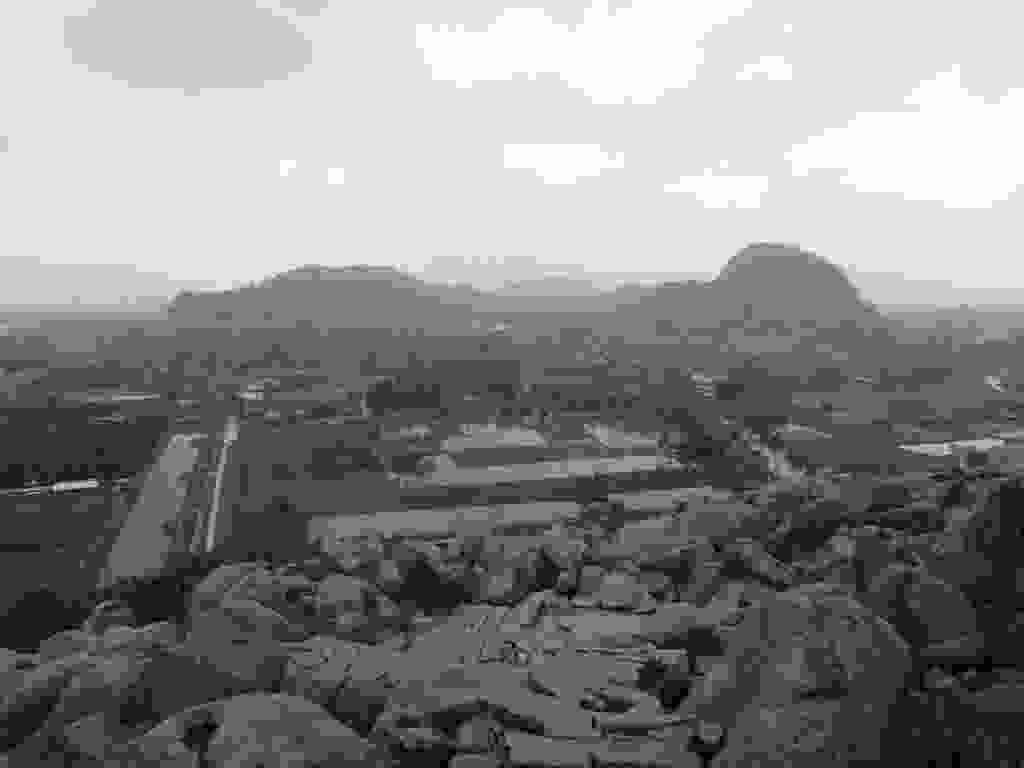
\includegraphics[width=\mywidth]{../wp-content/uploads/2015/12/wpid-oi000667-1024x768.jpg} } 
 \newline
 \newline
\centerline{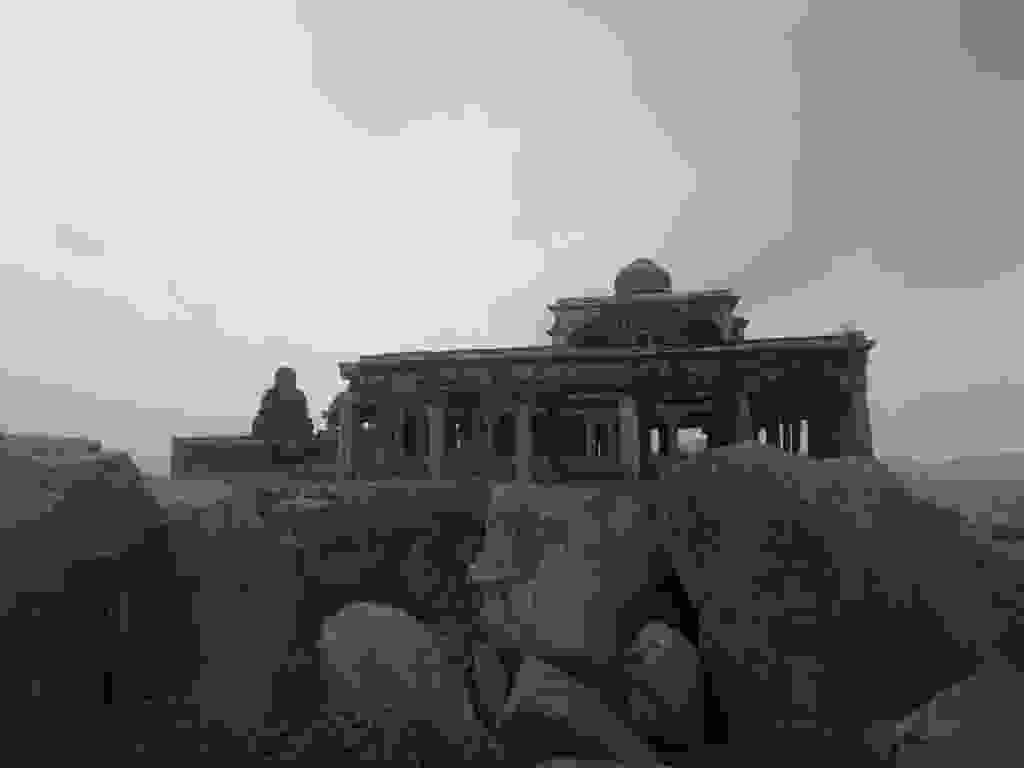
\includegraphics[width=\mywidth]{../wp-content/uploads/2015/12/wpid-oi000674-1024x768.jpg} } 
 \newline
 \newline
\centerline{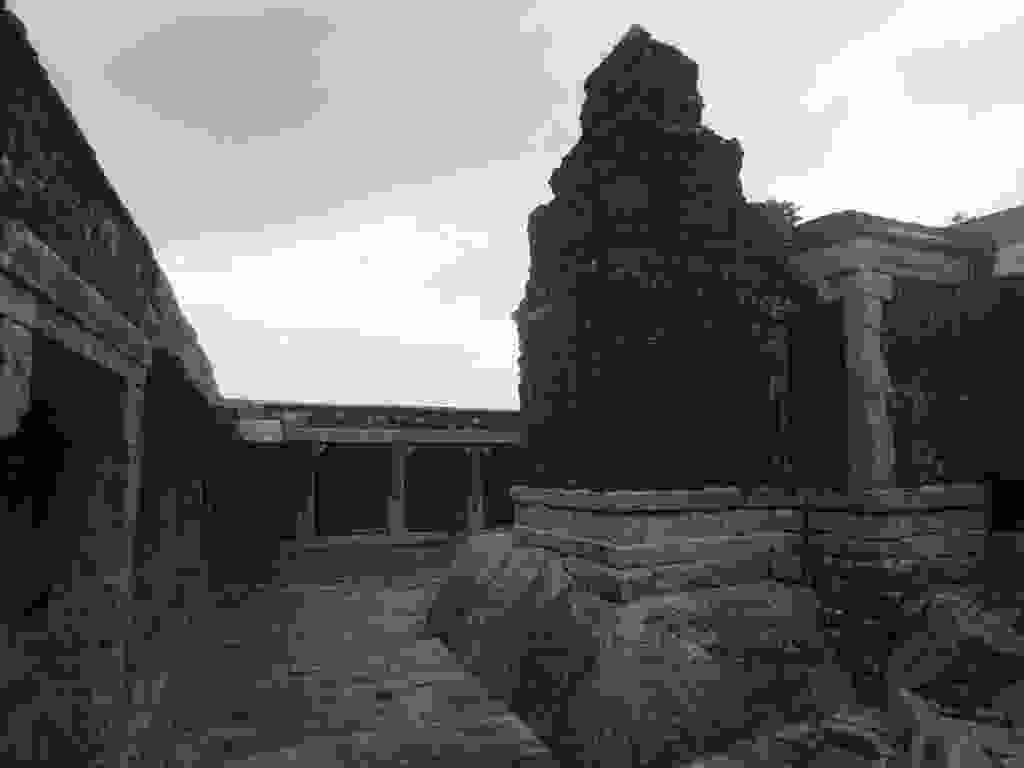
\includegraphics[width=\mywidth]{../wp-content/uploads/2015/12/wpid-oi000675-1024x768.jpg} } 
 \newline
 Puis 1 jour à Tiruvannamalai au pied de la montagne sacrée Arunachala, destination de pèlerinage \newline
 \newline
\centerline{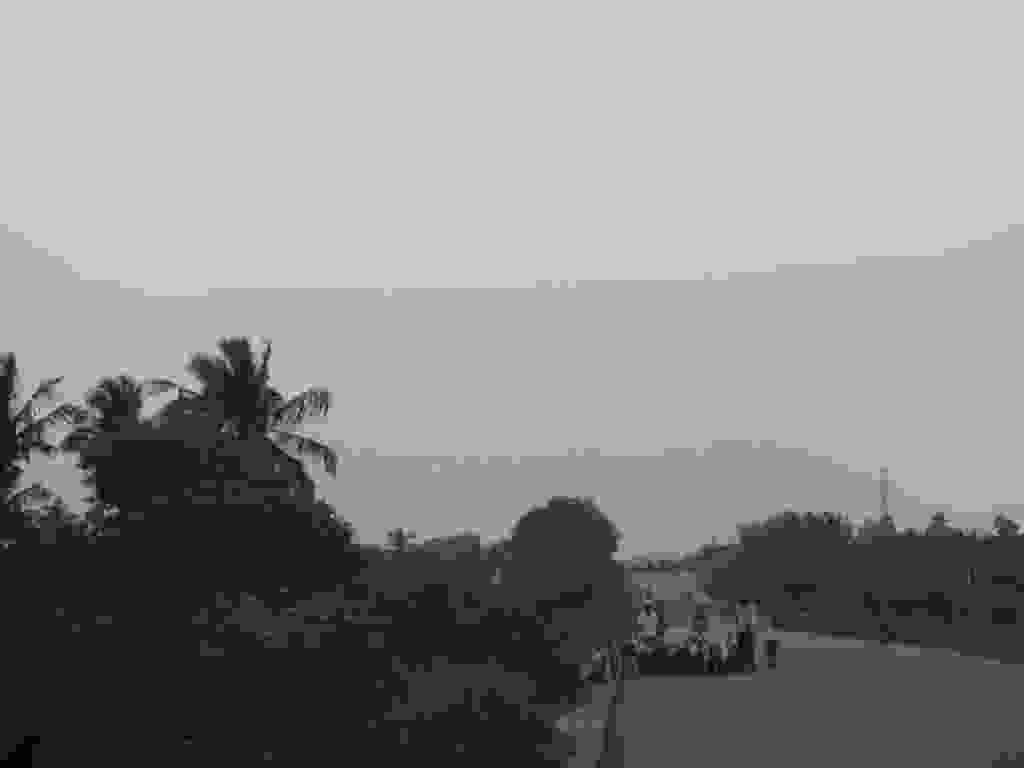
\includegraphics[width=\mywidth]{../wp-content/uploads/2015/12/wpid-oi000683-1024x768.jpg} } 
 \newline
 \newline
\centerline{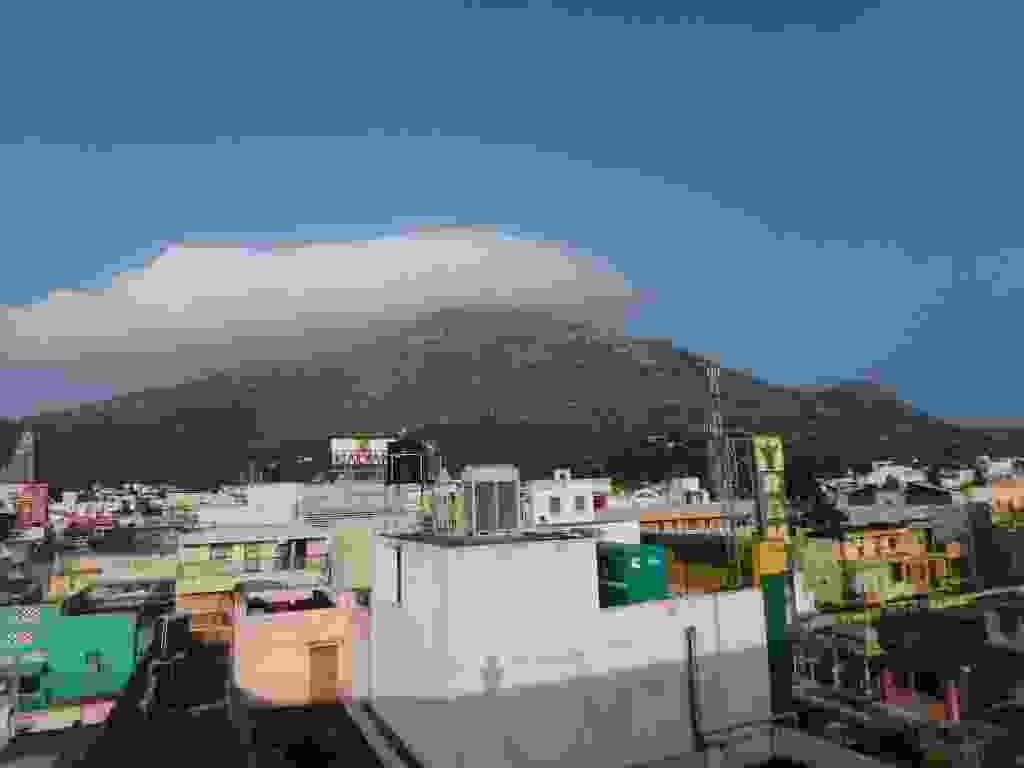
\includegraphics[width=\mywidth]{../wp-content/uploads/2015/12/wpid-oi000685-1024x768.jpg} } 
 \newline
 Temple Arunachaleswara \newline
 \newline
\centerline{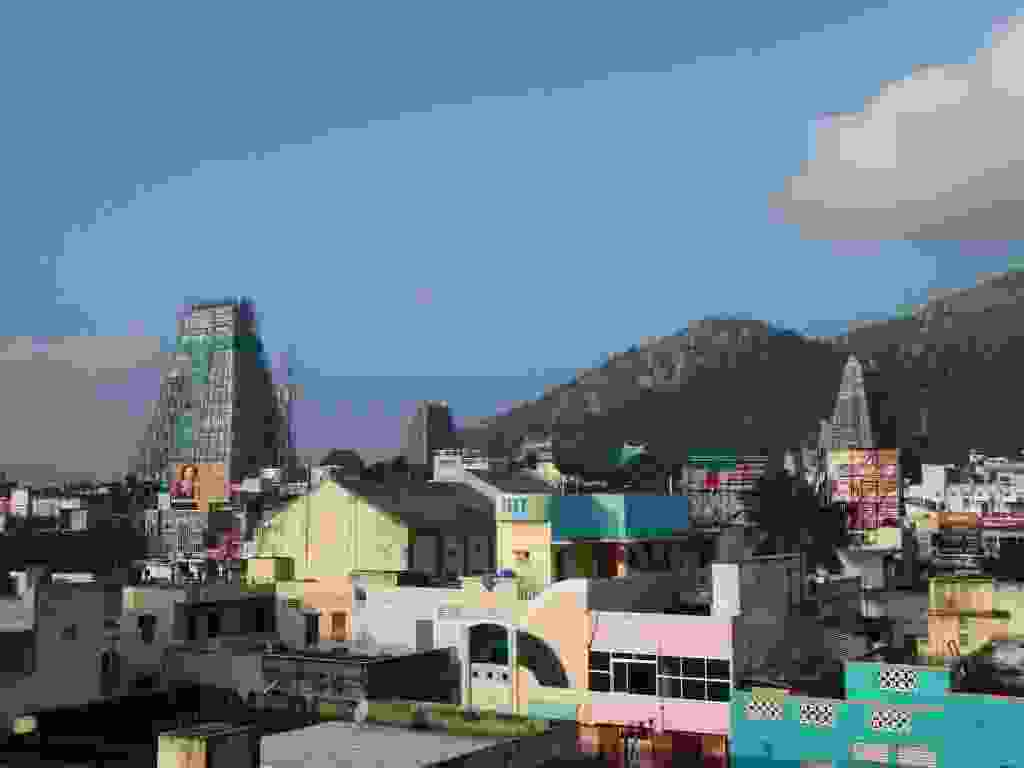
\includegraphics[width=\mywidth]{../wp-content/uploads/2015/12/wpid-oi000684-1024x768.jpg} } 
 \newline
 \newline
\centerline{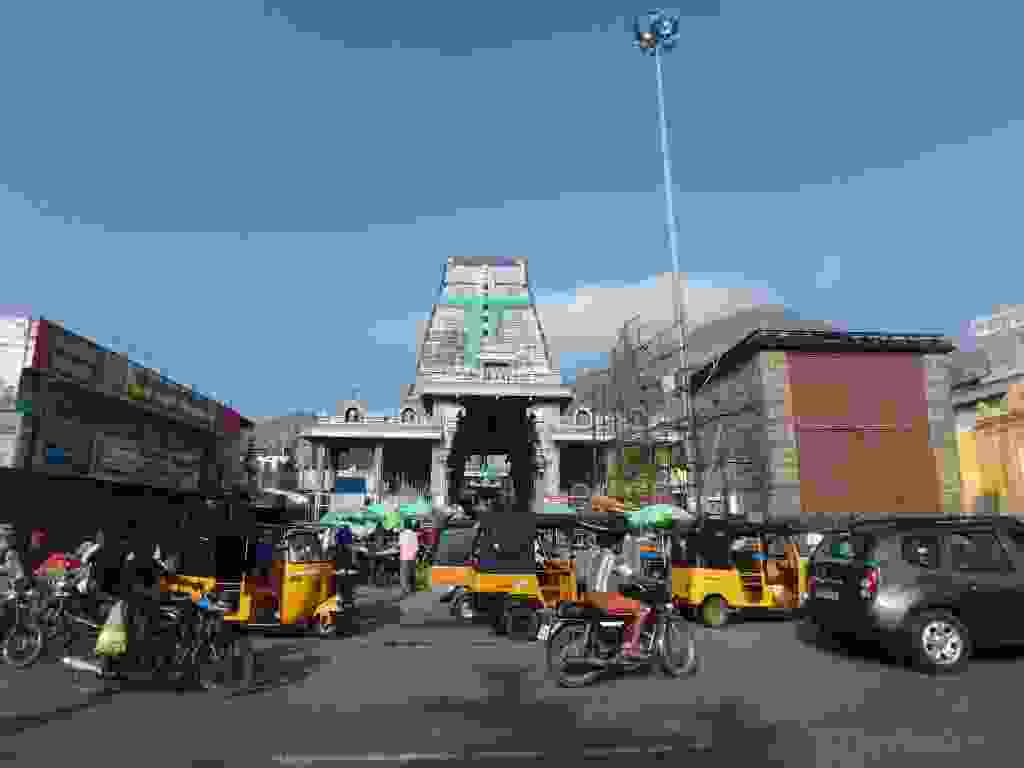
\includegraphics[width=\mywidth]{../wp-content/uploads/2015/12/wpid-oi000687-1024x768.jpg} } 
 \newline
 \newline
\centerline{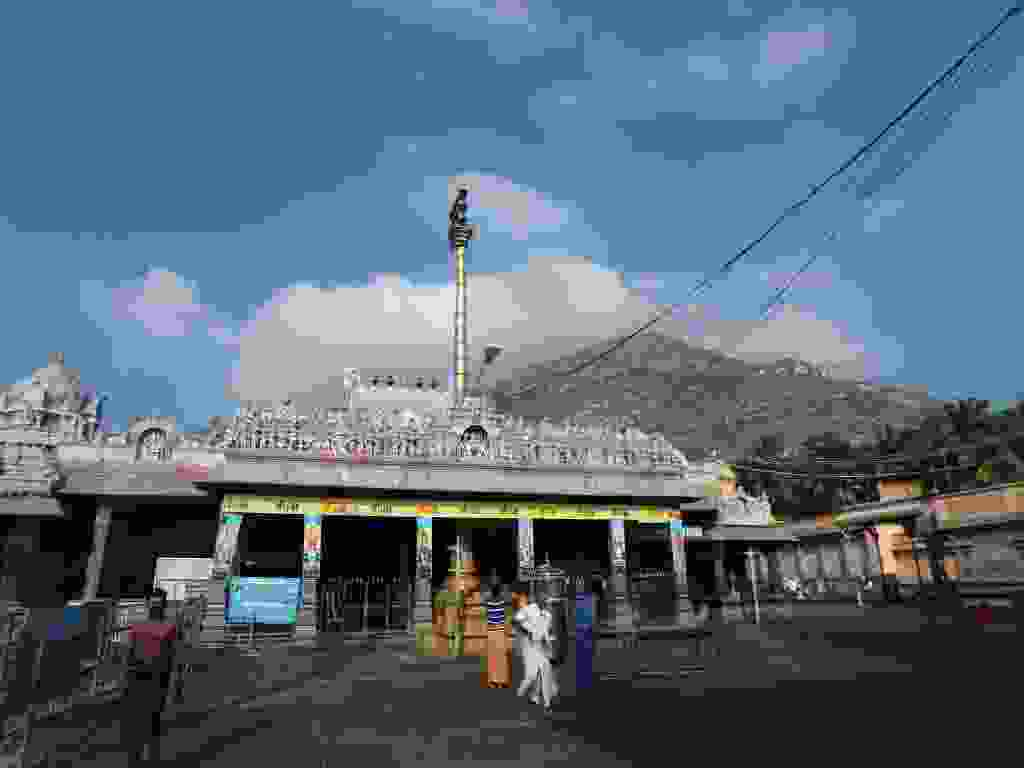
\includegraphics[width=\mywidth]{../wp-content/uploads/2015/12/wpid-oi000691-1024x768.jpg} } 
 \newline
 \newline
\centerline{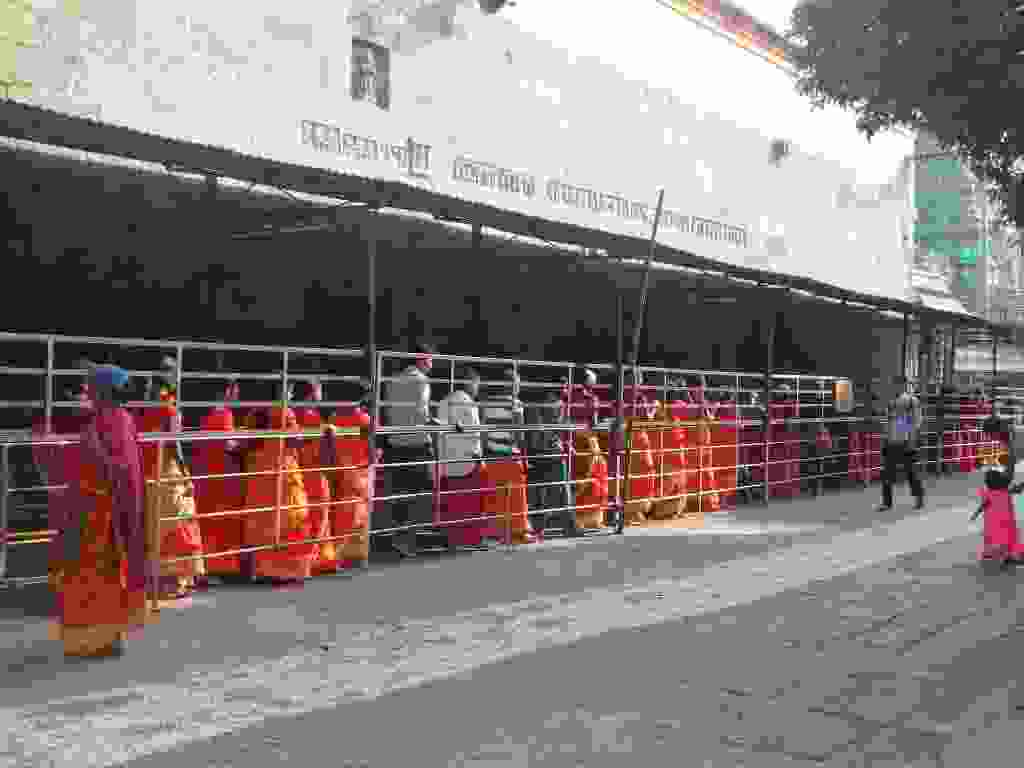
\includegraphics[width=\mywidth]{../wp-content/uploads/2015/12/wpid-oi000692-1024x768.jpg} } 
 \newline
 L'ashram du saint Ramana Maharishi, on peut entrer dans la grotte où il est resté en méditation pendant des années \newline
 \newline
\centerline{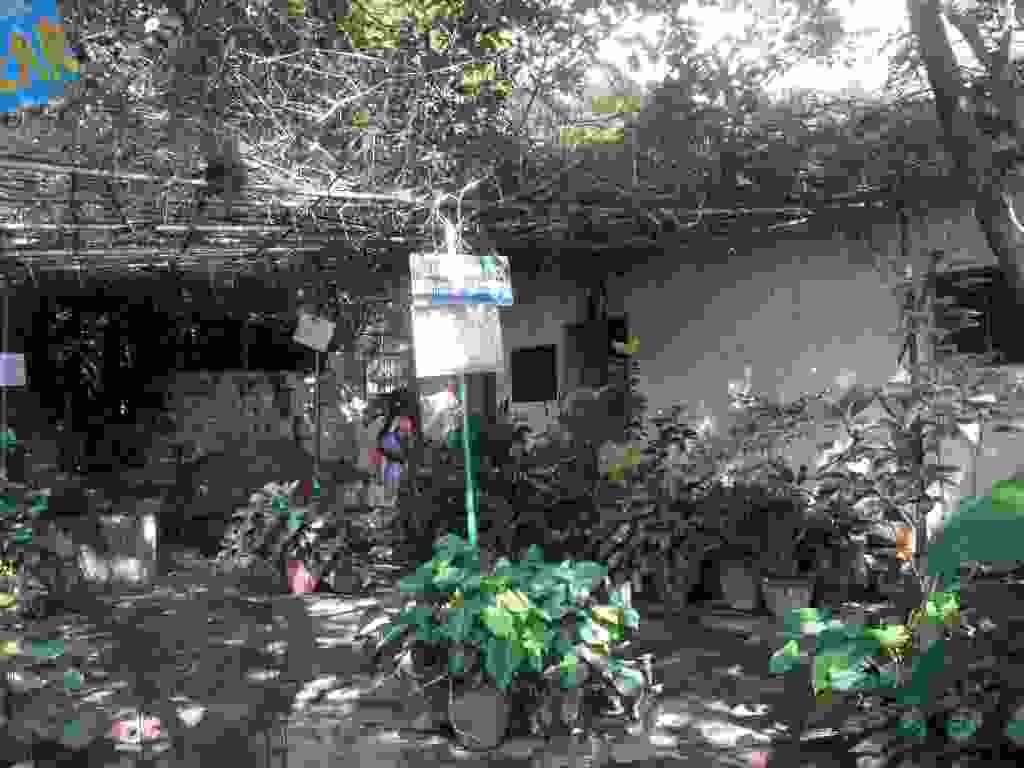
\includegraphics[width=\mywidth]{../wp-content/uploads/2015/12/wpid-oi000694-1024x768.jpg} } 
 \newline
 Montée au sommet de la montagne, un feu est entretenu en permanence \newline
 \newline
\centerline{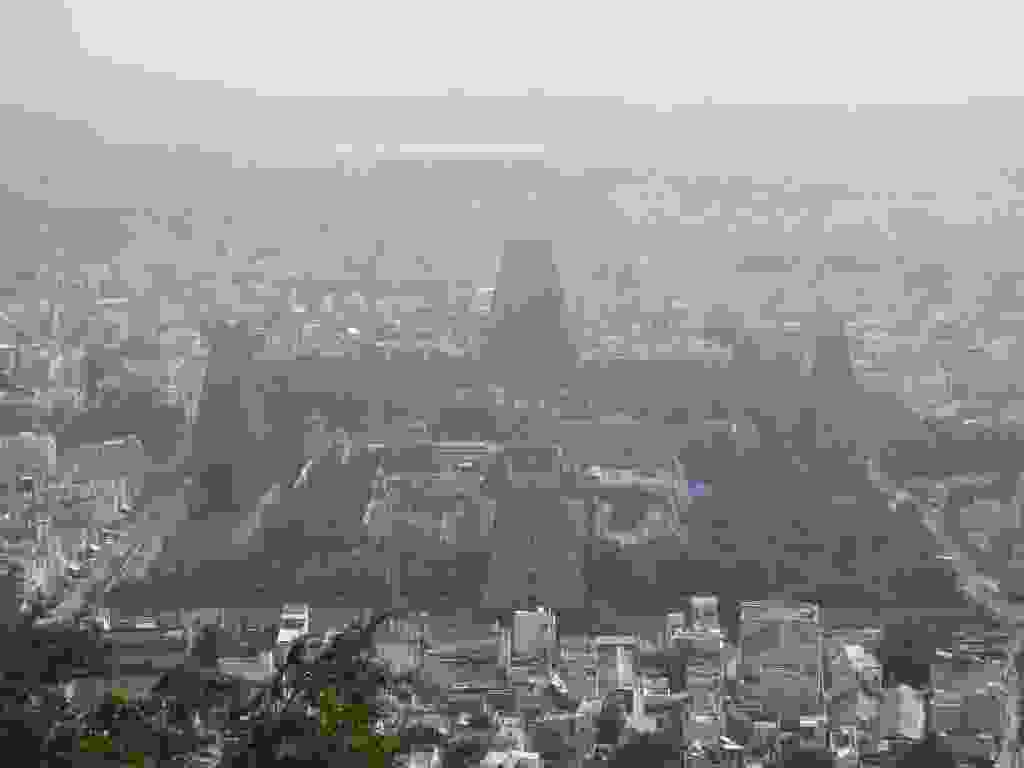
\includegraphics[width=\mywidth]{../wp-content/uploads/2015/12/wpid-oi000697-1024x768.jpg} } 
 \newline
 \newline
\centerline{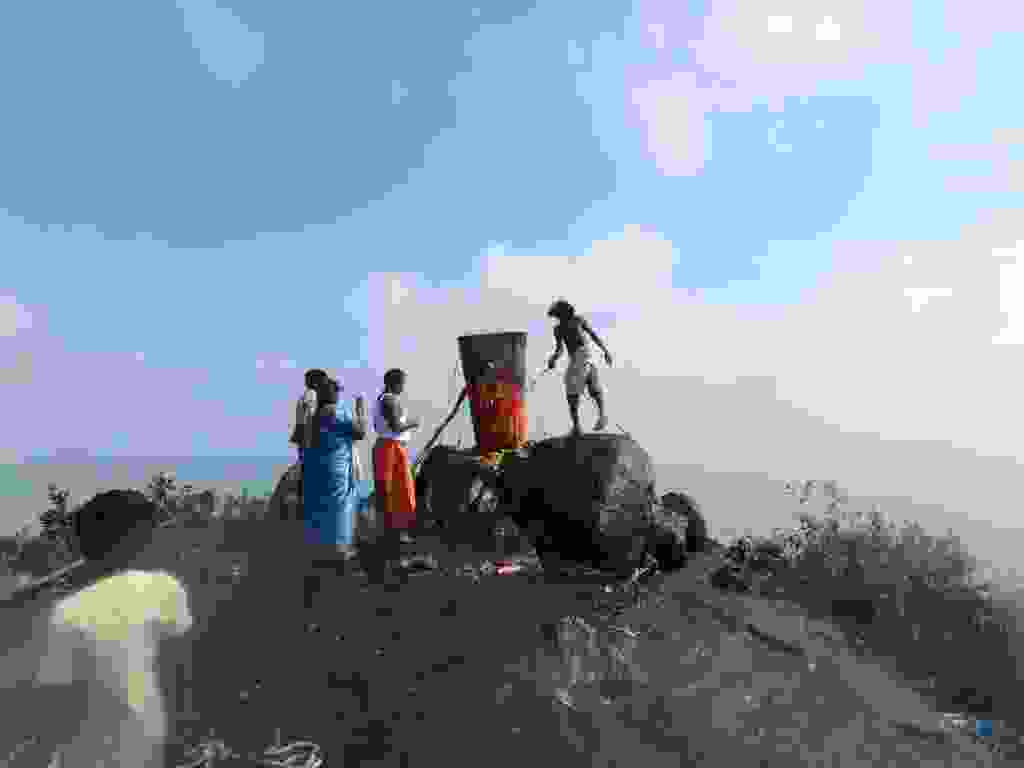
\includegraphics[width=\mywidth]{../wp-content/uploads/2015/12/wpid-oi000698-1024x768.jpg} } 
 \newline
 \newline
\centerline{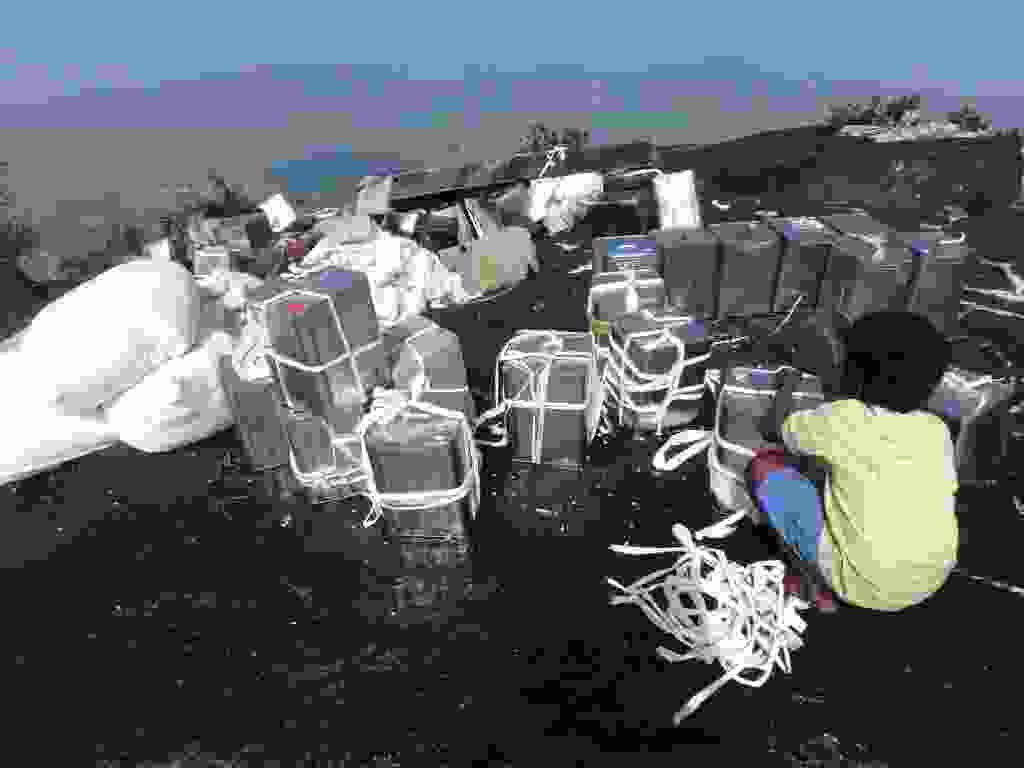
\includegraphics[width=\mywidth]{../wp-content/uploads/2015/12/wpid-oi000699-1024x768.jpg} } 
 \newline
 Chaque jour, des indiens en moto se mettent à côté de moi pour discuter pendant quelques centaines de mètres, parfois plusieurs km. \newline
 \newline
\centerline{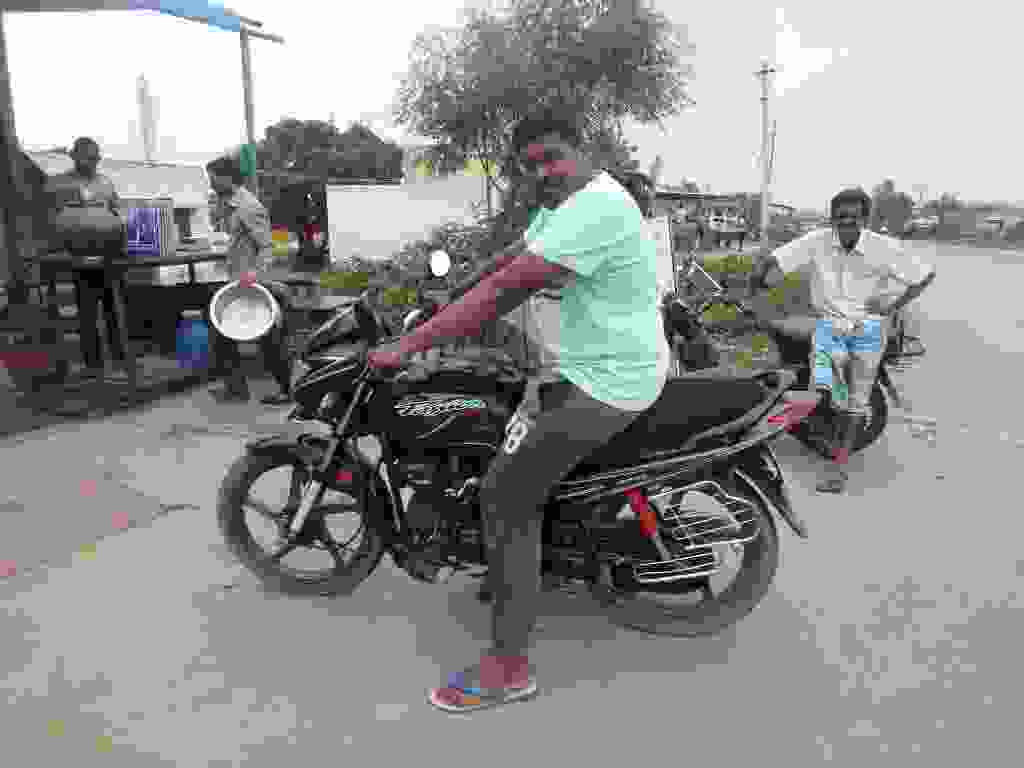
\includegraphics[width=\mywidth]{../wp-content/uploads/2015/12/wpid-oi000712-1024x768.jpg} } 
 \newline
 \newline
\centerline{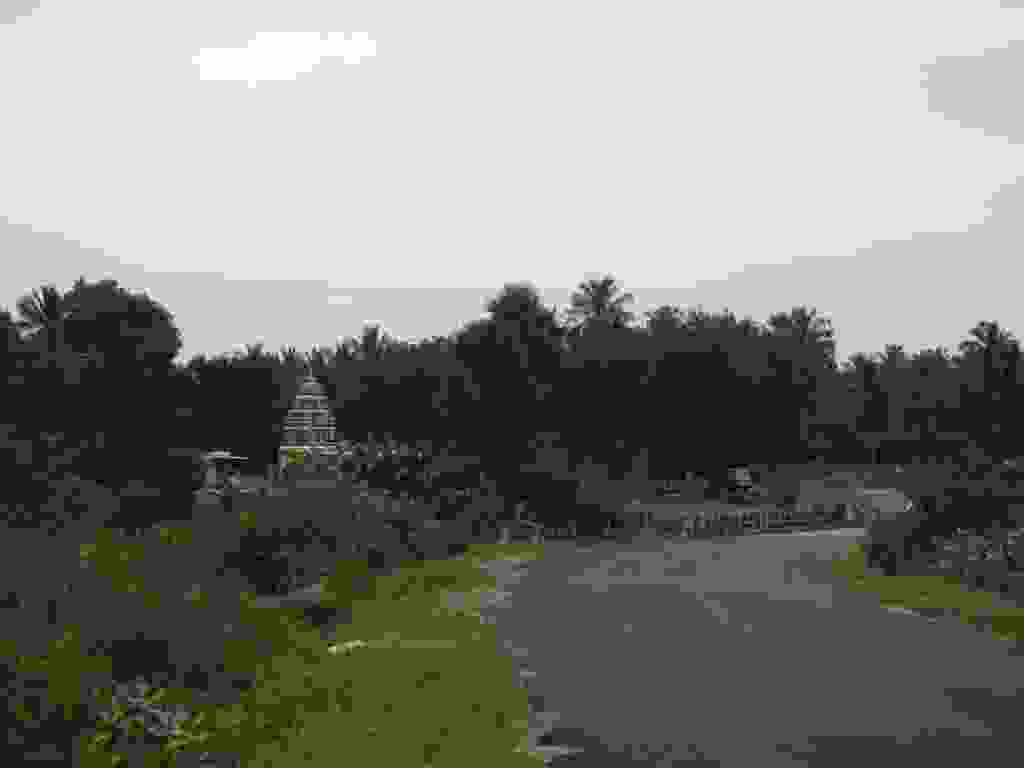
\includegraphics[width=\mywidth]{../wp-content/uploads/2015/12/wpid-oi000708-1024x768.jpg} } 
 \newline
 Dernière partie avant Bangalore sur l'autoroute \newline
 \newline
\centerline{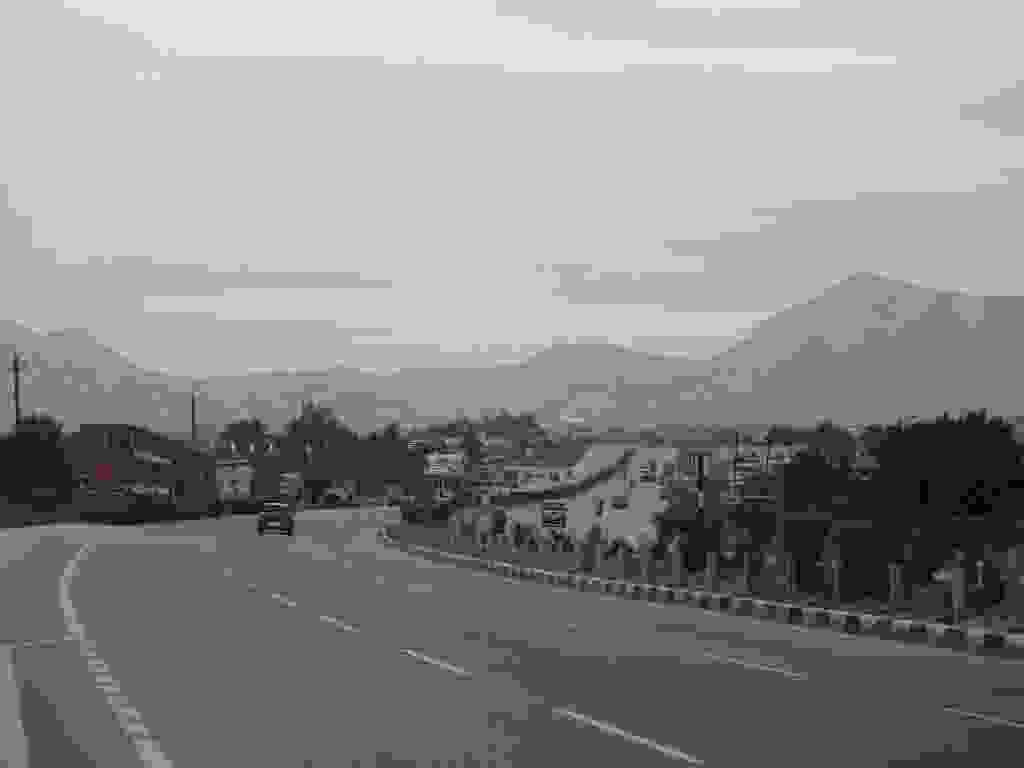
\includegraphics[width=\mywidth]{../wp-content/uploads/2015/12/wpid-oi000716-1024x768.jpg} } 
 \newline
 \newline
\centerline{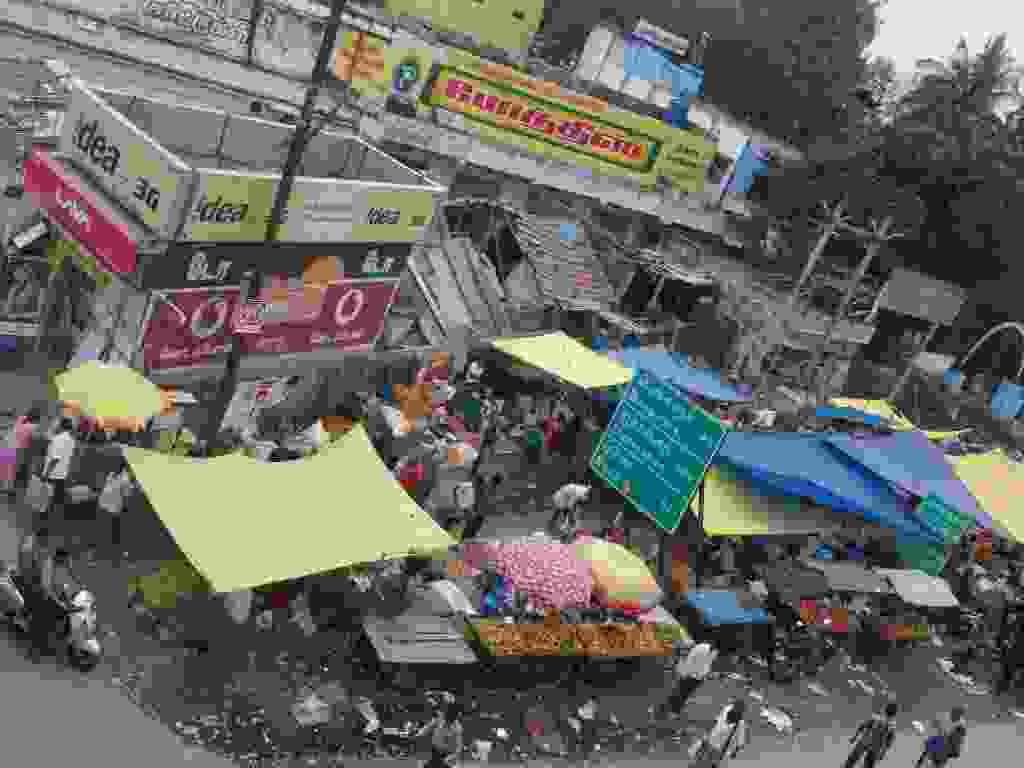
\includegraphics[width=\mywidth]{../wp-content/uploads/2015/12/wpid-oi000718-1024x768.jpg} } 
 \newline
 Centre de Bangalore, assez propre et moderne mais circulation énorme \newline
 \newline
\centerline{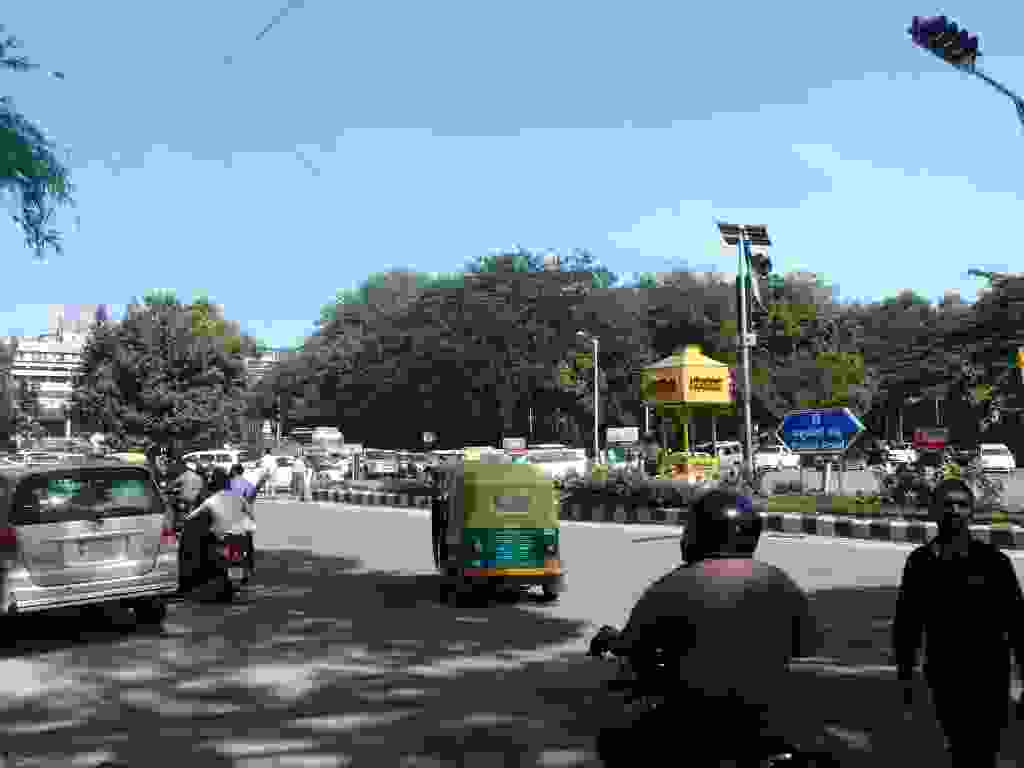
\includegraphics[width=\mywidth]{../wp-content/uploads/2015/12/wpid-oi000724-1024x768.jpg} } 
 \newline
 \newline
\centerline{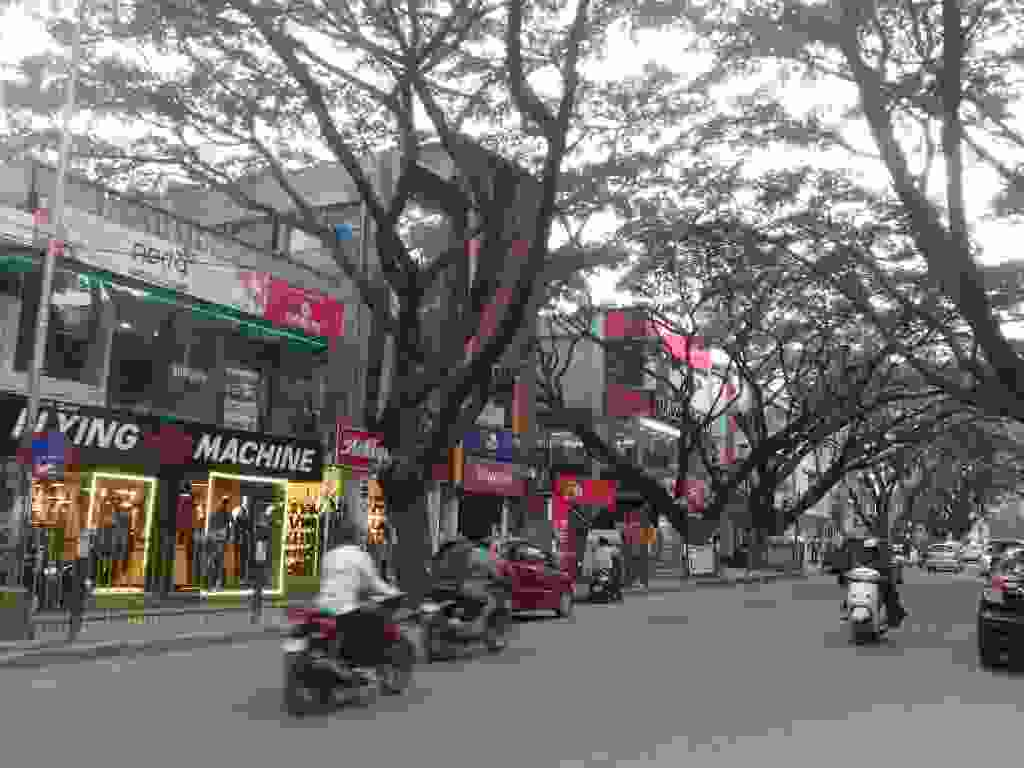
\includegraphics[width=\mywidth]{../wp-content/uploads/2015/12/wpid-oi000721-1024x768.jpg} } 
 \newline
 \newline
\centerline{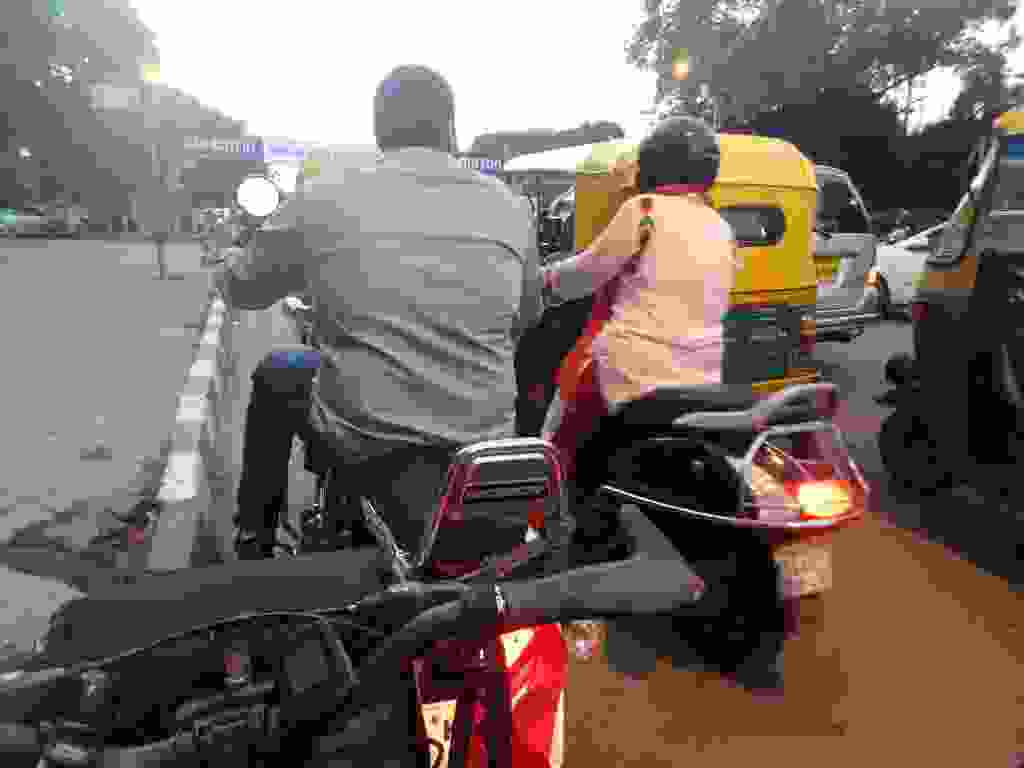
\includegraphics[width=\mywidth]{../wp-content/uploads/2015/12/wpid-oi000727-1024x768.jpg} } 
 \newline
 Maintenant plus que 2 semaines de voyage : ça sera vers le nord et sans le vélo \newline

\newpage
 
